\begin{figure}
\begin{tabular}{cc}
\begin{subfigure}[b]{0.52\textwidth}
\begin{center}
\begin{allLangEnvFoot}
~{\tiny \textcolor{mygray}{S0:}}~ OptStr strchr (Str s, i8 c) {
~{\tiny \textcolor{mygray}{S1:}}~   while ${\tt true}$:
~{\tiny \textcolor{mygray}{S2:}}~     assume ${\tt \neg (s\ is\ SInvalid)}$;
~{\tiny \textcolor{mygray}{S3:}}~     if s is SNil:
~{\tiny \textcolor{mygray}{S4:}}~       if c = ${\tt 0_{i8}}$: return Found(s);
~{\tiny \textcolor{mygray}{S5:}}~       return NotFound();
~{\tiny \textcolor{mygray}{S6:}}~     i8 ch $\coloneqq$ s.ch; // (s is SCons)
~{\tiny \textcolor{mygray}{S7:}}~     if c = ch: return Found(s);
~{\tiny \textcolor{mygray}{S8:}}~     s $\coloneqq$ s.tail;
~{\tiny \textcolor{mygray}{SE:}}~ }
\end{allLangEnvFoot}
\end{center}
\caption{\label{fig:llStrchrSpecIR}Strchr Specification}
\end{subfigure}%
&
\begin{subfigure}[b]{0.46\textwidth}
\begin{center}
\begin{allLangEnvFoot}
~{\tiny \textcolor{mygray}{\ \ \ }}~ char* strchr(char* t, int c);
~{\tiny \textcolor{mygray}{}}~
~{\tiny \textcolor{mygray}{C0:}}~ i32 strchr (i32 t, i32 c) {
~{\tiny \textcolor{mygray}{C1:}}~   i8 ch $\coloneqq$ c[7:0];
~{\tiny \textcolor{mygray}{C2:}}~   while $\arrIndex{\tt t}{0_{i32}}{\mem{}}{i8}$ $\neq$ ch:
~{\tiny \textcolor{mygray}{C3:}}~     if $\arrIndex{\tt t}{0_{i32}}{\mem{}}{i8}$ = $0_{i8}$:
~{\tiny \textcolor{mygray}{C4:}}~       return ${\tt 0_{i32}}$;
~{\tiny \textcolor{mygray}{C5:}}~     t $\coloneqq$ t + ${\tt 1_{i32}}$
~{\tiny \textcolor{mygray}{C6:}}~   return t;
~{\tiny \textcolor{mygray}{CE:}}~ }
\end{allLangEnvFoot}
\end{center}
\caption{\label{fig:llStrchrCArrIR}Strchr Implementation using Array}
\end{subfigure}%
\\
\begin{subfigure}[b]{0.52\textwidth}
\begin{center}
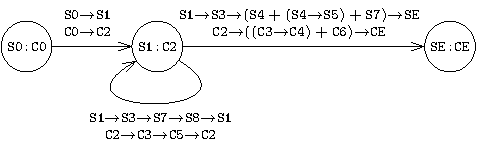
\includegraphics[scale=1.05]{chapters/figures/figStrchrProductCfg.pdf}
\end{center}
\vspace{2ex}
\caption{\label{fig:llStrchrProductCFG}Product CFG for programs \cref{fig:llStrchrSpecIR,fig:llStrchrCArrIR}}
\end{subfigure}%
&
\begin{subfigure}[b]{0.46\textwidth}
\begin{center}
\begin{footnotesize}
\begin{tabular}{|c|l|}
\hline
{\bf PC-Pair} & \multicolumn{1}{c|}{\bf Invariants} \\
\hline
\hline
\multirow{2}{*}{(\scpc{0}{0})} &
\Tstrut $\circled{\scriptsize P1} \  \sv{s} \indEq{} \lifted{str}{\mem{}}{u8[]}{\cv{t}}$ \\ &
\Tstrut $\circled{\scriptsize P2} \  \sv{c} = \cv{c}[7:0]$ \\
\multirow{2}{*}{(\scpc{1}{2})} &
\Tstrut $\circled{I1} \  \sv{s} \indEq{} \lifted{str}{\mem{}}{u8[]}{\cv{t}}$ \\ &
\Tstrut $\circled{I2} \  \sv{c} = \cv{ch}$ \\
(\scpc{E}{E}) &
\Tstrut \Bstrut $\circled{E} \  \sv{ret} \indEq{} \lifted{optstr}{\mem{}}{u8[]}{\cv{ret}}$ \\
\hline
\end{tabular}
\end{footnotesize}
\end{center}
\caption{\label{fig:llStrchrInvs}Invariants table for \cref{fig:llStrchrProductCFG}}
\end{subfigure}%
\\
\end{tabular}
\caption{\label{fig:llStrchrSpecAndCAndCFGAndInvs}\Cref{fig:llStrchrSpecIR,fig:llStrchrCArrIR} shows the (abstracted) IRs of \SpecL{} specification and a generic array-based C implementation.
\Cref{fig:llStrchrProductCFG} presents the Product-CFG showing a bisimulation relation between \cref{fig:llStrchrSpecIR,fig:llStrchrCArrIR}.
The node invariants for the product-CFG in \cref{fig:llStrchrProductCFG} are shown in \cref{fig:llStrchrInvs}.}
\end{figure}